\documentclass[12pt]{article}
\usepackage{enumerate}
\usepackage{notes}
\usepackage{oxford}

\begin{document}

\section{2017}

\subsection*{}  % 1
\begin{mdframed}
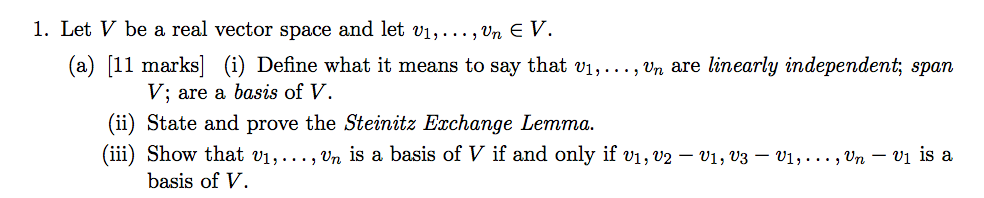
\includegraphics[width=400pt]{img/oxford-prelims-2017-A-1-1.png}
\end{mdframed}

\subsubsection*{(i)}
\begin{definition*}[Linear independence]
  Let $a_1, \ldots, a_n \in \R$. Then $v_1, v_2, \ldots, v_n$ are linearly
  independent if and only if the only solution to $\sum_{i=1}^n a_iv_i = 0$ is
  $a_1 = a_2 = \ldots = a_n = 0$.
\end{definition*}

\begin{definition*}[Span]
  $v_1, v_2, \ldots, v_n$ span $V$ if and only if for all $w \in V$ there exist
  $a_1, \ldots, a_n \in \R$ such that $\sum_{i=1}^n a_iv_i = w$.
\end{definition*}

\begin{definition*}[Basis]
  $v_1, v_2, \ldots, v_n$ are a basis for $V$ if and only if they span $V$ and
  they are linearly independent.
\end{definition*}

\subsubsection*{}
\begin{mdframed}
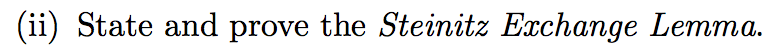
\includegraphics[width=250pt]{img/oxford-prelims-2017-A-1-1-2.png}
\end{mdframed}

\newpage
\begin{theorem*}[Steinitz Exchange Lemma - version 1]
  Let $X$ be a subset of a vector space $V$. Let $u \in \Span X$. Let $v \in X$
  be such that $u \notin \Span\(X \setminus \{v\}\)$. Then
  $\Span\(\(X \setminus \{v\}\) \cup \{u\}\) = \Span X$.
\end{theorem*}

[Informally: Take a set of vectors, one of which is $v$. Suppose their span
contains $u$, but, after removing $v$, their span no longer contains $u$. Now
consider the set resulting after exchanging $u$ for $v$. The span of this set
is the same as that of the original.]

\begin{proof}~\\
  Let $X$ be $\{v_1, \ldots, v_n\}$, and let $u \in \Span X$.

  Reorder the $v_i$ such that $u \notin \Span~ \{v_2, \ldots, v_n\}$.

  Note that $u = \sum_{i=1}^n\gamma_iv_i$ for some
  $\gamma_1, \ldots, \gamma_n \in \R$, where $\gamma_1 \neq 0$.

  Therefore $v_1 = \frac{1}{\gamma_1}\(u - \sum_{i=2}^n\gamma_iv_i\)$.

  So we have $u \in \Span~ \{v_1, \ldots, v_n\}$ and
  $v_1 \in \Span~ \{u, v_2, \ldots, v_n\}$.

  It is clear that any vector in $\Span~ \{u, v_2, \ldots, v_n\}$ can be
  rewritten as a linear combination of $\{v_1, \ldots, v_n\}$, and conversely
  that any vector in $\Span~ \{v_1, \ldots, v_n\}$ can be rewritten as a linear
  combination of $\{u, v_2, \ldots, v_n\}$ which proves the theorem
  \footnote{
    For the forwards direction, let $w$ be in $\Span~ \{u, v_2, \ldots, v_n\}$ we
    want to show that this implies $w \in \Span~ \{v_1, \ldots, v_n\}$.

    We have $w = au + \sum_{i=2}^n\lambda_iv_i$ for some
    $a, \lambda_2, \ldots, \lambda_n \in \R$, and therefore
    $$
      w = a\sum_{i=1}^n\gamma_iv_i + \sum_{i=2}^n\lambda_iv_i
        = a\gamma_1v_1 + \sum_{i=2}^n(\gamma_i + \lambda_i)v_i,
    $$
    proving that $w \in \Span~ \{v_1, \ldots, v_n\}$, as required.~\\

    For the reverse direction, let $w$ be in $\Span~ \{v_1, \ldots, v_n\}$; we want
    to show that this implies $w \in \Span~ \{u, v_2, \ldots, v_n\}$. We have $w = \sum_{i=1}^n\lambda_iv_i$ for some
    $a, \lambda_2, \ldots, \lambda_n \in \R$, and therefore
    $$
      w = \frac{\lambda_1}{\gamma_1}\(u - \sum_{i=2}^n\gamma_iv_i\) + \sum_{i=2}^n\lambda_iv_i
        = \frac{\lambda_1}{\gamma_1}u + \sum_{i=2}^n(\lambda_i - \gamma_i)v_i,
    $$
    proving that $w \in \Span~ \{u, v_2, \ldots, v_n\}$, as required.
  }.

\end{proof}

\newpage
\begin{theorem*}
  A linearly independent set can be no larger than a spanning set.
\end{theorem*}

\begin{proof}
  Let $V$ be a vector space.

  Let $i_1, \ldots, i_m \in V$ be linearly independent.

  Let $s_1, \ldots, s_n \in V$ span $V$.

  Suppose for a contradiction that $m > n$.


\end{proof}

\begin{theorem*}
  Every basis has the same size.
\end{theorem*}

\begin{theorem*}
  A spanning set that is the same size as a basis is also a basis.
\end{theorem*}



\newpage
\subsubsection*{}
\begin{mdframed}
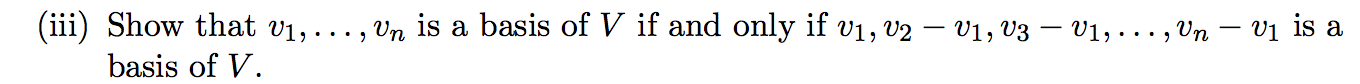
\includegraphics[width=400pt]{img/oxford-prelims-2017-A-1-1-3.png}
\end{mdframed}


\begin{proof}~\\
$\implies$\\
For the forward implication, suppose that $v_1, \ldots, v_n$ is a basis of $V$.

Then for all $w \in V$ there exist unique coordinates $\lambda_1, \ldots, \lambda_n$ such that
\begin{align*}
  \sum_{i=1}^n \lambda_iv_i &= w.
\end{align*}
Subtracting $\(\sum_{i=1}^n \lambda_i\)v_1$ from both sides we have
\begin{align*}
  \sum_{i=1}^n \lambda_i(v_i - v_1) &= w - \(\sum_{i=1}^n \lambda_i\)v_1\\
  \(\sum_{i=1}^n \lambda_i\)v_1 + \sum_{i=2}^n \lambda_i(v_i - v_1) &= w,
\end{align*}
proving that $v_1, v_2 - v_1, \ldots, v_n - v_1$ spans $V$.

Furthermore, $v_1, v_2 - v_1, \ldots, v_n - v_1$ are linearly independent,
since a corollary of the Steinitz Exchange Lemma is that if a spanning set is
the same size as a linearly independent set, then the spanning set is also
linearly independent (and the linearly independent set spans, so in fact both
are bases).

$\impliedby$\\
For the reverse implication, suppose that $v_1, v_2 - v_1, \ldots, v_n - v_1$
is a basis of $V$.

Then for all $w \in V$ there exist unique coordinates $\lambda_1, \ldots, \lambda_n$ such that
\begin{align*}
  \lambda_1v_1 + \sum_{i=2}^n \lambda_i(v_i - v_1) = w.
\end{align*}
Equivalently,
\begin{align*}
  \Big(\lambda_1 - \sum_{i=2}^n\lambda_i\Big)v_1 + \sum_{i=2}^n \lambda_iv_i = w,
\end{align*}

proving that $v_1, v_2, \ldots, v_n$ span $V$.

Furthermore, $v_1, v_2, \ldots, v_n$ are linearly independent, by the same
Steinitz Exchange Lemma argument given above.
\end{proof}

~\\
\newpage
\begin{mdframed}
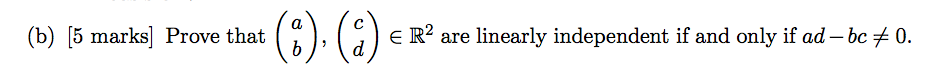
\includegraphics[width=400pt]{img/oxford-prelims-2017-A-1-2.png}
\end{mdframed}

\renewcommand{\cvec}[2]{\begin{pmatrix}#1\\#2\end{pmatrix}}

\begin{proof}
Let $x_1 = \cvec{a}{b}$ and $x_2 = \cvec{c}{d}$

We prove the negation; that $x_1, x_2$ linearly dependent is equivalent to
$ad - bc = 0$.

$\implies$\\
For the forwards implication, we prove that $x_1, x_2$ linearly dependent
implies $ad - bc = 0$.

Since they are linearly dependent, there exists $\lambda_1, \lambda_2 \in \R$
such that $\lambda_1x_1 + \lambda_2x_2 = 0$, with at least one of
$\lambda_1, \lambda_2$ non-zero.

Suppose, without loss of generality, that $\lambda_1 = 0$. Then
$\lambda_2 \neq 0$ and therefore $c = d = 0$, and therefore $ad - bc = 0$.

The remaining case is that $\lambda_1 \neq 0$ and $\lambda_2 \neq 0$. Then
\begin{align*}
  \begin{cases}
    a\lambda_1 + c\lambda_2 = 0\\
    b\lambda_1 + d\lambda_2 = 0,
  \end{cases}
\end{align*}
therefore
\begin{align*}
  \lambda_1                            &= -\frac{c}{a}\lambda_2\\
  \Big(-\frac{bc}{a} + d\Big)\lambda_2 &= 0\\
  ad - bc                              &= 0.
\end{align*}

$\impliedby$\\
For the reverse implication, we prove that $ad - bc = 0$ implies $x_1, x_2$
linearly dependent.

\red{TODO: Not sure how to do this without resorting to properties of
  determinant of linear transformation.}

Let $u_1, u_2$ be a basis for $\R^2$ and consider the matrix
$\mat{a}{c} {b}{d}$ with respect to this basis.

Viewed as a linear transformation, the matrix sends $u_1 \mapsto x_1$ and
$u_2 \mapsto x_2$.

The determinant of this matrix is $ad - bc$. Since the determinant is zero, the
linear transformation maps the basis vectors into a one- or zero-dimensional
subspace.

Therefore $x_1,x_2$ lie in a one dimensional subspace. Therefore
$x_1 = \lambda x_2$ for some $\lambda \in \R$. Therefore $x_1,x_2$ are linearly
dependent.

\end{proof}

\begin{mdframed}
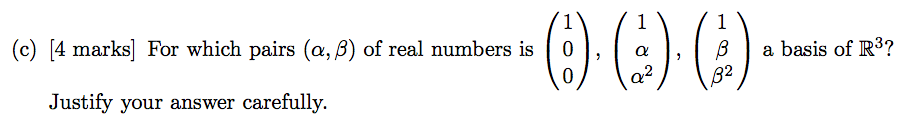
\includegraphics[width=400pt]{img/oxford-prelims-2017-A-1-3.png}
\end{mdframed}

\red{TODO}

\subsection*{}  % 2
\begin{mdframed}
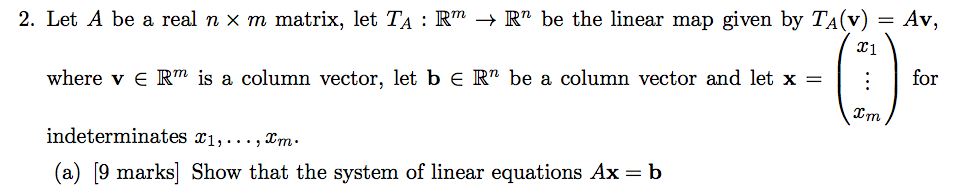
\includegraphics[width=400pt]{img/oxford-prelims-2017-A-2-1.png}
\end{mdframed}

\subsection*{}  % 2.a.i
\begin{mdframed}

\includegraphics[width=400pt]{img/oxford-prelims-2017-A-2-1-1.png}
\end{mdframed}

By definition,  $\im T_A = \{Ax: x \in \R^m\}$.

Let $S$ denote the proposition ``$Ax = b$ has a solution''.

By the definition of ``has a solution'', $S$ is equivalent to the proposition
``there exists $x \in \R^m$ such that $Ax = b$''.

We see that $S \implies b \in \im T_A$, and also that $b \in \im T_A \implies S$.

\subsubsection*{} % 2.a.ii
\begin{mdframed}
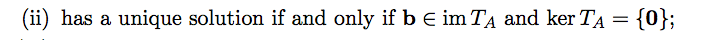
\includegraphics[width=400pt]{img/oxford-prelims-2017-A-2-1-2.png}
\end{mdframed}

Let $S_u$ denote the proposition ``$Ax = b$ has a unique solution''.

First we prove the forwards implication:

\begin{claim*}
  $S_u \implies \Big(b \in \im T_A ~~\text{and}~~ \ker T_A = \{0\}\Big)$.
\end{claim*}

\begin{proof}
Firstly, since $S_u \implies S$, we know from part (i) that
$S_u \implies b \in \Im T_A$.

Suppose $S_u$ is true and let $x$ be the unique solution.

We know that $0 \in \ker A$ since $A(0) = A(x - x) = Ax - Ax = 0$ by the
linearity of $A$.

Now suppose there exists $y \neq 0 \in \ker T_A$. But
\begin{align*}
A(x + y) = Ax + Ay = b + 0 = b,
\end{align*}
so $x + y \neq x$ is also a solution; a contradiction. Therefore no such $y$
exists and we see that $S_u \implies \ker T_A = \{0\}$.
\end{proof}

Now we prove the reverse implication:

\begin{claim*}
  $\Big(b \in \Im T_A ~~\text{and}~~ \ker T_A = \{0\}\Big) \implies S_u$.
\end{claim*}

\begin{proof}
  Suppose $b \in \Im T_A$. Then we know from part (i) that $S$ is true. So let
  $x$ be a solution.

Now suppose that $\ker T_A = \{0\}$ and that $y \neq x$ is another solution. But then
\begin{align*}
  A(x - y) = Ax - Ay = b - b = 0,
\end{align*}
so $x - y \neq 0 \in \ker T_A$; a contradiction. Therefore if $\ker T_A = \{0\}$
then no such $y$ exists.
\end{proof}

\subsubsection*{} % 2.a.iii
\begin{mdframed}
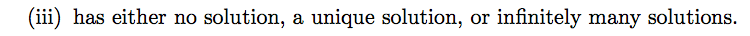
\includegraphics[width=400pt]{img/oxford-prelims-2017-A-2-1-3.png}
\end{mdframed}

Suppose $Ax = b$ has $n > 1$ solutions and let the first two such solutions be
$x_1$ and $x_2$. Then there are uncountably infinitely many solutions, since
for all $\alpha \in \R$
\begin{align*}
A\Big(x_1 + \alpha (x_2 - x_1)\Big) = Ax_1 + \alpha(Ax_2 - Ax_1) = b + \alpha(b - b) = b.
\end{align*}

\subsection*{} % 2.b
\begin{mdframed}
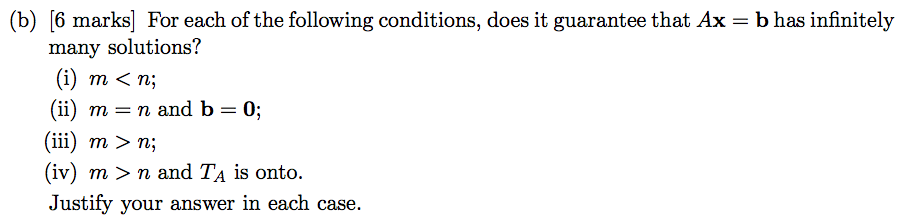
\includegraphics[width=400pt]{img/oxford-prelims-2017-A-2-2.png}
\end{mdframed}

\subsubsection*{(i)} The mapping takes vectors in a lower dimensional space and
outputs vectors in a higher dimensional space. E.g. suppose $T_A:\R^1 \to \R^2$
and let $A = \scvec{s}{t}$. Then $Ax = (xs, xt)$ i.e. $\Im T_A$ is a line
through the origin.

\begin{align*}
  m &=    \dim(\ker T_A) + \dim(\im T_A)\\
    &\leq \dim(\ker T_A) + n\\
\end{align*}
~\\
\subsection*{} % 2.c
\begin{mdframed}
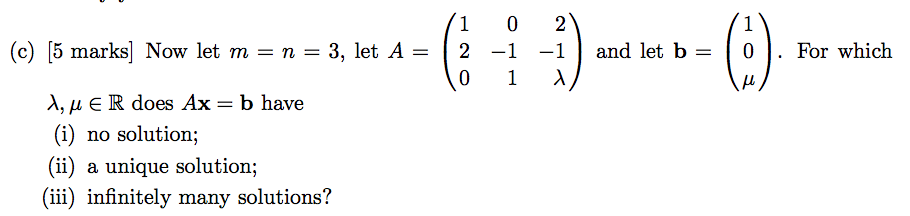
\includegraphics[width=400pt]{img/oxford-prelims-2017-A-2-3.png}
\end{mdframed}

\end{document}
